\documentclass[hidelinks,12pt]{article}

\usepackage[italian]{babel}
\usepackage[a4paper]{geometry}
\usepackage{amsmath, tikz, hyperref, caption, subcaption, circuitikz}
\usepackage[capitalize, italian]{cleveref}
\usepackage[
   backend=biber,
   style=numeric,
 ]{biblatex}
\addbibresource{bib/db.bib}

% -- Font settings
\usepackage[math-style=ISO]{unicode-math}
\setmainfont{EB Garamond}%You should have installed the font
\setmathfont{Garamond-Math.otf}[StylisticSet={8,9}]
\setmathfont{Garamond-Math.otf}[range={scr,bfscr}]

\setlength{\parskip}{1.2ex}
\setlength{\parindent}{0em}
\clubpenalty = 100
\widowpenalty = 100

\title{STM32 GameBoy}
\date{\today}
\author{Marco Cutecchia, Edoardo Marangoni \\
\footnotesize \texttt{\{marco.cutecchia, edoardo.marangoni1\}@studenti.unimi.it} \\ }

\begin{document}
\maketitle

\section{Introduzione}
Il GameBoy è una console portatile rilasciata da Nintendo all'inizio degli anni
90 che diede inizio al grandissimo successo dei videogiochi tascabili.
La console vendette più di 118 milioni di unità nel mondo e divenne un fenomeno
culturale ricordato ancora oggi.

Lo scopo del progetto è quello di costruire un'imitazione del GameBoy in grado
di giocare tutti i videogiochi originali, ma con una serie di miglioramenti
grazie ai componenti hardware più moderni. Tra le modifiche al dispositivo
originale che abbiamo implementato troviamo il caricamento dei giochi tramite
microSD, invece che con cartucce, e l'utilizzo di uno schermo a colori e
retroilluminato, al contrario dell'originale schermo a scala di grigi che
diventava impossibile da vedere sotto scarsa luce.

\section{Hardware}
Le componenti hardware utilizzate sono tre: una scheda basata sul
SoC \texttt{STM32F411CEU6} (\cref{fig:weact_blackpill}),
uno schermo TFT da $2.4"$ basata sul controllore \texttt{ILI9341}
(\cref{fig:ili9341}) ed infine una PCB per la plancia di gioco clone
dell'originale utilizzata nel GameBoy (\cref{fig:pcb}).
Non è stato necessario comprare un lettore di schede microSD perchè il
display scelto ne integra uno al suo interno.

Oltre a questi componenti attivi sono stati utilizzati un interruttore SPDT,
dei pulsanti in plastica ed i rispettivi gommini da posizionare sopra la PCB
dei tasti, delle millefori (insieme a stagno, cavi e pin) per costruire i
collegamenti in modo da minimizzare lo spazio utilizzato ed infine un case di
GameBoy dove è stato alloggiato il tutto.

La componente centrale del progetto è il microcontrollore
\texttt{STM32F411CEU6}, prodotto da ST e montato sulla board \texttt{WeAct Black
	Pill V2.0}. Il microcontrollore monta un core \texttt{ARM} Cortex-M4 con clock
massimo di $100$MHz (overclockato a $140$). Questo microcontrollore offre $34$
pin GPIO che verranno utilizzati per collegare il microcontrollore a schermo e
pad; monta $512$KiB di memoria flash e $128$KiB di SRAM, necessari per
l'esecuzione del software che abbiamo utilizzato.
\begin{figure}
	\begin{subfigure}[b]{0.45\textwidth}
		\begin{center}
			\begin{tikzpicture}[x=0.015cm, y=0.015cm, scale=0.5, transform shape]
					\draw  [color={rgb, 255:red, 0; green, 0; blue, 0 }  ,draw opacity=1 ][fill={rgb, 255:red, 255; green, 255; blue, 255 }  ,fill opacity=1 ] (480,140) -- (640,140) -- (640,960) -- (480,960) -- cycle ;
	\draw  [fill={rgb, 255:red, 255; green, 255; blue, 255 }  ,fill opacity=1 ] (440,150) -- (510,150) -- (510,190) -- (440,190) -- cycle ;
	\draw  [fill={rgb, 255:red, 255; green, 255; blue, 255 }  ,fill opacity=1 ] (440,190) -- (510,190) -- (510,230) -- (440,230) -- cycle ;
	\draw  [fill={rgb, 255:red, 255; green, 255; blue, 255 }  ,fill opacity=1 ] (440,230) -- (510,230) -- (510,270) -- (440,270) -- cycle ;
	\draw  [fill={rgb, 255:red, 255; green, 255; blue, 255 }  ,fill opacity=1 ] (440,270) -- (510,270) -- (510,310) -- (440,310) -- cycle ;
	\draw  [fill={rgb, 255:red, 255; green, 255; blue, 255 }  ,fill opacity=1 ] (440,310) -- (510,310) -- (510,350) -- (440,350) -- cycle ;
	\draw  [fill={rgb, 255:red, 255; green, 255; blue, 255 }  ,fill opacity=1 ] (440,350) -- (510,350) -- (510,390) -- (440,390) -- cycle ;
	\draw  [fill={rgb, 255:red, 255; green, 255; blue, 255 }  ,fill opacity=1 ] (440,390) -- (510,390) -- (510,430) -- (440,430) -- cycle ;
	\draw  [fill={rgb, 255:red, 255; green, 255; blue, 255 }  ,fill opacity=1 ] (440,430) -- (510,430) -- (510,470) -- (440,470) -- cycle ;
	\draw  [fill={rgb, 255:red, 255; green, 255; blue, 255 }  ,fill opacity=1 ] (440,470) -- (510,470) -- (510,510) -- (440,510) -- cycle ;
	\draw  [fill={rgb, 255:red, 255; green, 255; blue, 255 }  ,fill opacity=1 ] (440,510) -- (510,510) -- (510,550) -- (440,550) -- cycle ;
	\draw  [fill={rgb, 255:red, 255; green, 255; blue, 255 }  ,fill opacity=1 ] (440,550) -- (510,550) -- (510,590) -- (440,590) -- cycle ;
	\draw  [fill={rgb, 255:red, 255; green, 255; blue, 255 }  ,fill opacity=1 ] (440,630) -- (510,630) -- (510,670) -- (440,670) -- cycle ;
	\draw  [fill={rgb, 255:red, 255; green, 255; blue, 255 }  ,fill opacity=1 ] (440,670) -- (510,670) -- (510,710) -- (440,710) -- cycle ;
	\draw  [fill={rgb, 255:red, 255; green, 255; blue, 255 }  ,fill opacity=1 ] (440,710) -- (510,710) -- (510,750) -- (440,750) -- cycle ;
	\draw  [fill={rgb, 255:red, 255; green, 255; blue, 255 }  ,fill opacity=1 ] (440,750) -- (510,750) -- (510,790) -- (440,790) -- cycle ;
	\draw  [fill={rgb, 255:red, 255; green, 255; blue, 255 }  ,fill opacity=1 ] (440,790) -- (510,790) -- (510,830) -- (440,830) -- cycle ;
	\draw  [fill={rgb, 255:red, 255; green, 255; blue, 255 }  ,fill opacity=1 ] (440,830) -- (510,830) -- (510,870) -- (440,870) -- cycle ;
	\draw  [fill={rgb, 255:red, 255; green, 255; blue, 255 }  ,fill opacity=1 ] (440,870) -- (510,870) -- (510,910) -- (440,910) -- cycle ;
	\draw  [fill={rgb, 255:red, 255; green, 255; blue, 255 }  ,fill opacity=1 ] (440,910) -- (510,910) -- (510,950) -- (440,950) -- cycle ;
	\draw  [fill={rgb, 255:red, 255; green, 255; blue, 255 }  ,fill opacity=1 ] (610,150) -- (680,150) -- (680,190) -- (610,190) -- cycle ;
	\draw  [fill={rgb, 255:red, 255; green, 255; blue, 255 }  ,fill opacity=1 ] (610,190) -- (680,190) -- (680,230) -- (610,230) -- cycle ;
	\draw  [fill={rgb, 255:red, 255; green, 255; blue, 255 }  ,fill opacity=1 ] (610,230) -- (680,230) -- (680,270) -- (610,270) -- cycle ;
	\draw  [fill={rgb, 255:red, 255; green, 255; blue, 255 }  ,fill opacity=1 ] (610,270) -- (680,270) -- (680,310) -- (610,310) -- cycle ;
	\draw  [fill={rgb, 255:red, 255; green, 255; blue, 255 }  ,fill opacity=1 ] (610,310) -- (680,310) -- (680,350) -- (610,350) -- cycle ;
	\draw  [fill={rgb, 255:red, 255; green, 255; blue, 255 }  ,fill opacity=1 ] (610,350) -- (680,350) -- (680,390) -- (610,390) -- cycle ;
	\draw  [fill={rgb, 255:red, 255; green, 255; blue, 255 }  ,fill opacity=1 ] (610,390) -- (680,390) -- (680,430) -- (610,430) -- cycle ;
	\draw  [fill={rgb, 255:red, 255; green, 255; blue, 255 }  ,fill opacity=1 ] (610,430) -- (680,430) -- (680,470) -- (610,470) -- cycle ;
	\draw  [fill={rgb, 255:red, 255; green, 255; blue, 255 }  ,fill opacity=1 ] (610,470) -- (680,470) -- (680,510) -- (610,510) -- cycle ;
	\draw  [fill={rgb, 255:red, 255; green, 255; blue, 255 }  ,fill opacity=1 ] (610,510) -- (680,510) -- (680,550) -- (610,550) -- cycle ;
	\draw  [fill={rgb, 255:red, 255; green, 255; blue, 255 }  ,fill opacity=1 ] (610,550) -- (680,550) -- (680,590) -- (610,590) -- cycle ;
	\draw  [fill={rgb, 255:red, 255; green, 255; blue, 255 }  ,fill opacity=1 ] (610,590) -- (680,590) -- (680,630) -- (610,630) -- cycle ;
	\draw  [fill={rgb, 255:red, 255; green, 255; blue, 255 }  ,fill opacity=1 ] (610,630) -- (680,630) -- (680,670) -- (610,670) -- cycle ;
	\draw  [fill={rgb, 255:red, 255; green, 255; blue, 255 }  ,fill opacity=1 ] (610,670) -- (680,670) -- (680,710) -- (610,710) -- cycle ;
	\draw  [fill={rgb, 255:red, 255; green, 255; blue, 255 }  ,fill opacity=1 ] (610,710) -- (680,710) -- (680,750) -- (610,750) -- cycle ;
	\draw  [fill={rgb, 255:red, 255; green, 255; blue, 255 }  ,fill opacity=1 ] (610,750) -- (680,750) -- (680,790) -- (610,790) -- cycle ;
	\draw  [fill={rgb, 255:red, 255; green, 255; blue, 255 }  ,fill opacity=1 ] (610,790) -- (680,790) -- (680,830) -- (610,830) -- cycle ;
	\draw  [fill={rgb, 255:red, 255; green, 255; blue, 255 }  ,fill opacity=1 ] (610,830) -- (680,830) -- (680,870) -- (610,870) -- cycle ;
	\draw  [fill={rgb, 255:red, 255; green, 255; blue, 255 }  ,fill opacity=1 ] (610,870) -- (680,870) -- (680,910) -- (610,910) -- cycle ;
	\draw  [fill={rgb, 255:red, 255; green, 255; blue, 255 }  ,fill opacity=1 ] (440,590) -- (510,590) -- (510,630) -- (440,630) -- cycle ;
	\draw  [fill={rgb, 255:red, 255; green, 255; blue, 255 }  ,fill opacity=1 ] (610,910) -- (680,910) -- (680,950) -- (610,950) -- cycle ;
	\draw (445,180) node [anchor=north west][inner sep=0.75pt]   [align=left] {$B12$};
	\draw (445,220) node [anchor=north west][inner sep=0.75pt]   [align=left] {$B13$};
	\draw (445,260) node [anchor=north west][inner sep=0.75pt]   [align=left] {$B14$};
	\draw (445,300) node [anchor=north west][inner sep=0.75pt]   [align=left] {$B15$};
	\draw (445,340) node [anchor=north west][inner sep=0.75pt]   [align=left] {$A8$};
	\draw (445,380) node [anchor=north west][inner sep=0.75pt]   [align=left] {$A9$};
	\draw (445,420) node [anchor=north west][inner sep=0.75pt]   [align=left] {$A10$};
	\draw (445,460) node [anchor=north west][inner sep=0.75pt]   [align=left] {$A11$};
	\draw (445,500) node [anchor=north west][inner sep=0.75pt]   [align=left] {$A12$};
	\draw (445,540) node [anchor=north west][inner sep=0.75pt]   [align=left] {$A15$};
	\draw (445,580) node [anchor=north west][inner sep=0.75pt]   [align=left] {$B3$};
	\draw (445,620) node [anchor=north west][inner sep=0.75pt]   [align=left] {$B4$};
	\draw (445,660) node [anchor=north west][inner sep=0.75pt]   [align=left] {$B5$};
	\draw (445,700) node [anchor=north west][inner sep=0.75pt]   [align=left] {$B6$};
	\draw (445,740) node [anchor=north west][inner sep=0.75pt]   [align=left] {$B7$};
	\draw (445,780) node [anchor=north west][inner sep=0.75pt]   [align=left] {$B8$};
	\draw (445,820) node [anchor=north west][inner sep=0.75pt]   [align=left] {$B9$};
	\draw (445,860) node [anchor=north west][inner sep=0.75pt]   [align=left] {$5V$};
	\draw (445,900) node [anchor=north west][inner sep=0.75pt]   [align=left] {$G$};
	\draw (445,940) node [anchor=north west][inner sep=0.75pt]   [align=left] {$3V3$};
	\draw (620,180) node [anchor=north west][inner sep=0.75pt]   [align=left] {$5V$};
	\draw (620,220) node [anchor=north west][inner sep=0.75pt]   [align=left] {$G$};
	\draw (620,260) node [anchor=north west][inner sep=0.75pt]   [align=left] {$3V3$};
	\draw (620,300) node [anchor=north west][inner sep=0.75pt]   [align=left] {$B10$};
	\draw (620,340) node [anchor=north west][inner sep=0.75pt]   [align=left] {$B2$};
	\draw (620,380) node [anchor=north west][inner sep=0.75pt]   [align=left] {$B1$};
	\draw (620,420) node [anchor=north west][inner sep=0.75pt]   [align=left] {$B0$};
	\draw (620,460) node [anchor=north west][inner sep=0.75pt]   [align=left] {$A7$};
	\draw (620,500) node [anchor=north west][inner sep=0.75pt]   [align=left] {$A6$};
	\draw (620,540) node [anchor=north west][inner sep=0.75pt]   [align=left] {$A5$};
	\draw (620,580) node [anchor=north west][inner sep=0.75pt]   [align=left] {$A4$};
	\draw (620,620) node [anchor=north west][inner sep=0.75pt]   [align=left] {$A3$};
	\draw (620,660) node [anchor=north west][inner sep=0.75pt]   [align=left] {$A2$};
	\draw (620,700) node [anchor=north west][inner sep=0.75pt]   [align=left] {$A1$};
	\draw (620,740) node [anchor=north west][inner sep=0.75pt]   [align=left] {$A0$};
	\draw (620,780) node [anchor=north west][inner sep=0.75pt]   [align=left] {$R$};
	\draw (620,820) node [anchor=north west][inner sep=0.75pt]   [align=left] {$C15$};
	\draw (620,860) node [anchor=north west][inner sep=0.75pt]   [align=left] {$C14$};
	\draw (620,900) node [anchor=north west][inner sep=0.75pt]   [align=left] {$C13$};
	\draw (620,940) node [anchor=north west][inner sep=0.75pt]   [align=left] {$VB$};

			\end{tikzpicture}
		\end{center}
		\caption{Pinout del microcontrollore STM32F411CEU6.}
		\label{fig:pinout_stm32}
	\end{subfigure}
	\hfill
	\begin{subfigure}[b]{0.45\textwidth}
		\begin{center}
			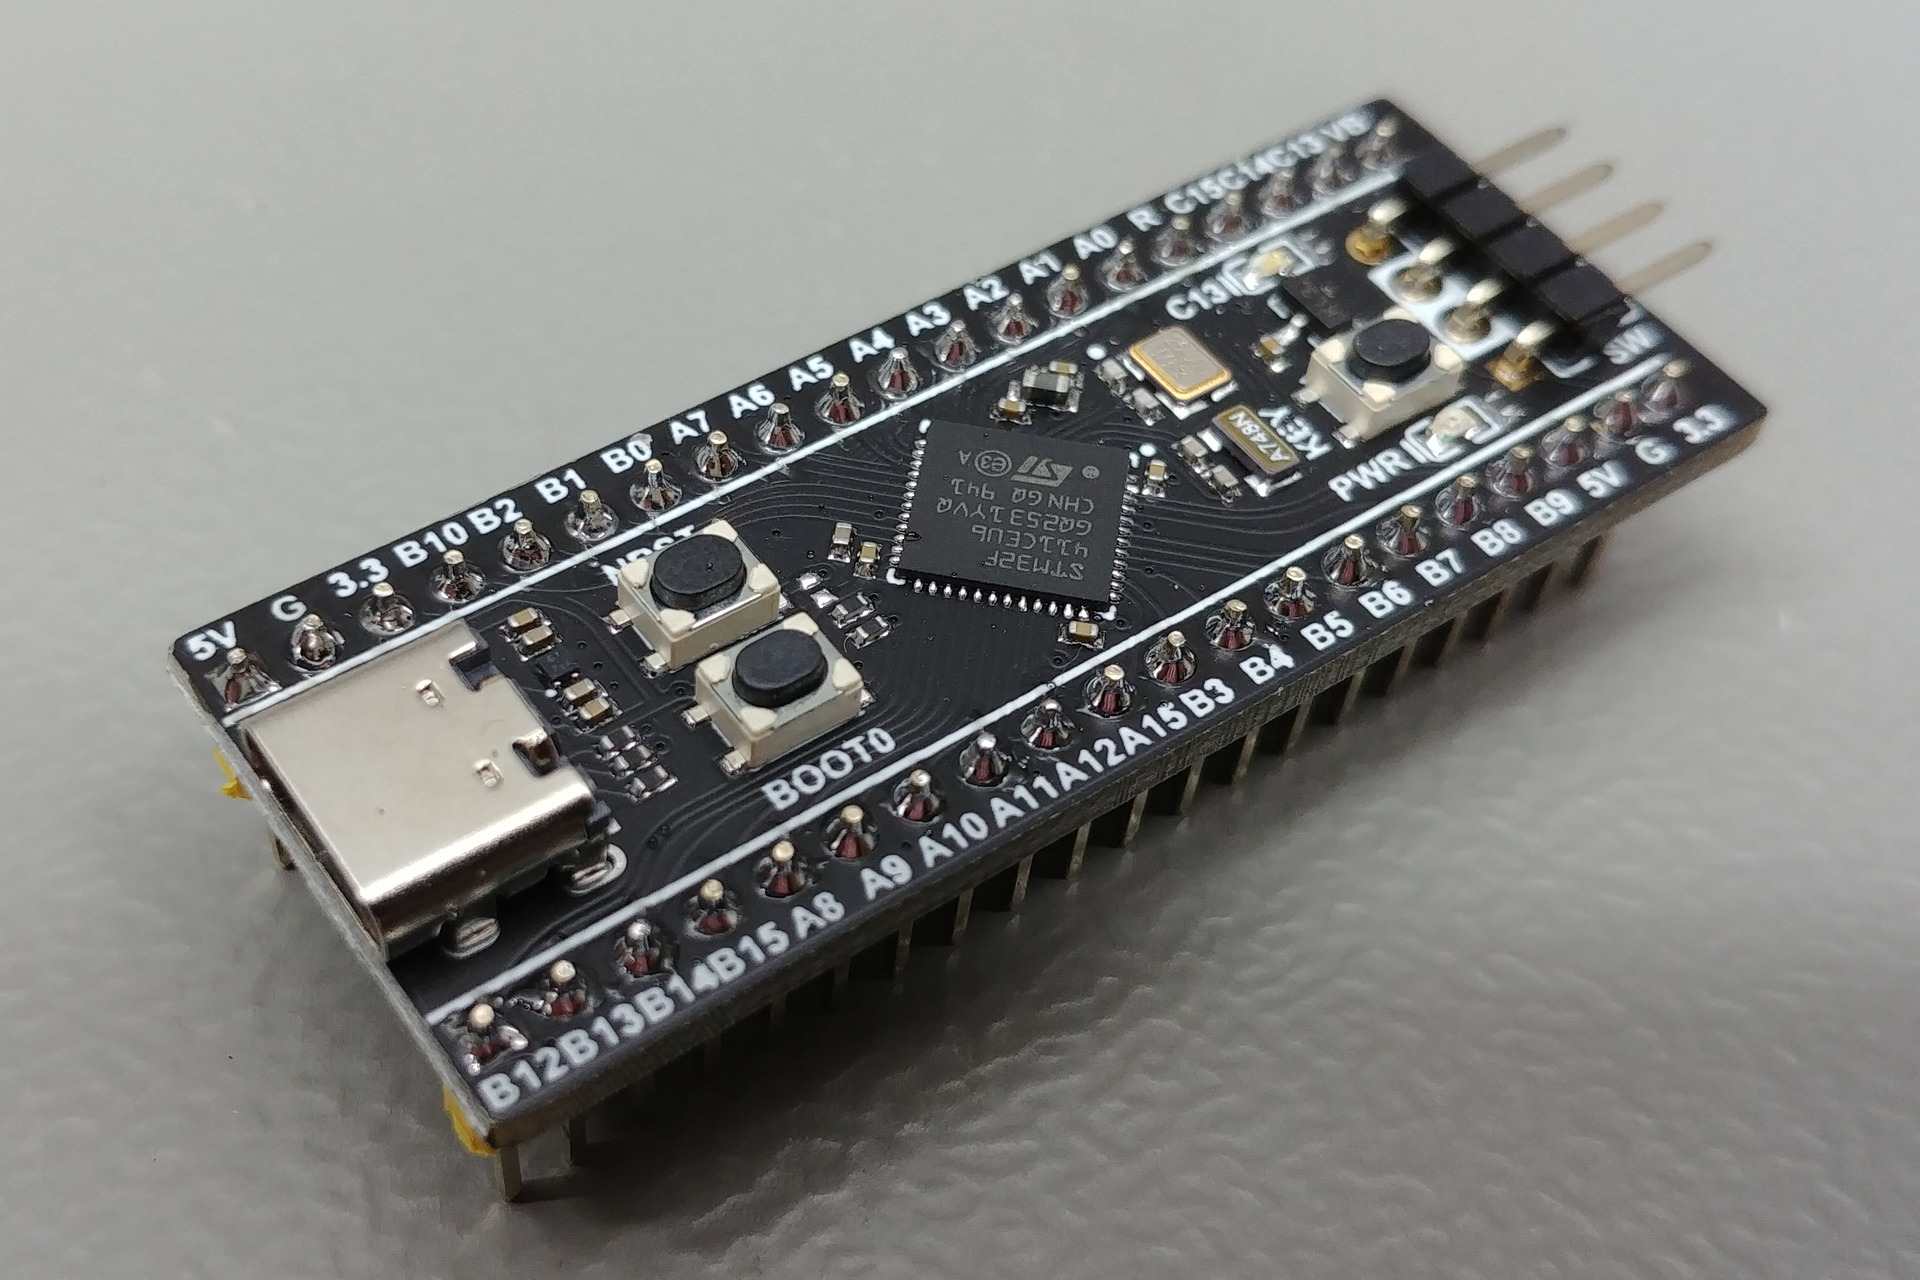
\includegraphics[scale=0.5]{figures/stm32.jpg}
		\end{center}
		\caption{La scheda \texttt{WeAct Black Pill V2.0}.}
		\label{fig:weact_blackpill}
	\end{subfigure}
\end{figure}

Lo schermo che abbiamo utilizzato, basato sul controller \texttt{ILI9341}, è
uno schermo LCD da $2.4"$, con una risoluzione di $320x240$ e controllo
individuale dei pixel, dotato di pin per il controllo dello schermo e della
microSD che si può inserire nella stessa board.
\begin{figure}[h]
	\begin{subfigure}[b]{0.45\textwidth}
		\begin{center}
			\begin{tikzpicture}[x=0.015cm, y=0.015cm, scale=0.5, transform shape]
				\draw   (120, 90) -- (320,90) -- (320,480) -- (120,480) -- cycle ;

\draw  [fill={rgb, 255:red, 255; green, 255; blue, 255 }  ,fill opacity=1 ]  (90,100)  --  (200,100) -- (200,130) --  (90,130) -- cycle;
\draw  [fill={rgb, 255:red, 255; green, 255; blue, 255 }  ,fill opacity=1 ]  (90,130)  --  (200,130) -- (200,160) --  (90,160) -- cycle;
\draw  [fill={rgb, 255:red, 255; green, 255; blue, 255 }  ,fill opacity=1 ]  (90,160)  --  (200,160) -- (200,190) --  (90,190) -- cycle;
\draw  [fill={rgb, 255:red, 255; green, 255; blue, 255 }  ,fill opacity=1 ]  (90,190)  --  (200,190) -- (200,220) --  (90,220) -- cycle;
\draw  [fill={rgb, 255:red, 255; green, 255; blue, 255 }  ,fill opacity=1 ]  (90,220)  --  (200,220) -- (200,250) --  (90,250) -- cycle;
\draw  [fill={rgb, 255:red, 255; green, 255; blue, 255 }  ,fill opacity=1 ]  (90,250)  --  (200,250) -- (200,280) --  (90,280) -- cycle;
\draw  [fill={rgb, 255:red, 255; green, 255; blue, 255 }  ,fill opacity=1 ]  (90,280)  --  (200,280) -- (200,310) --  (90,310) -- cycle;
\draw  [fill={rgb, 255:red, 255; green, 255; blue, 255 }  ,fill opacity=1 ]  (90,310)  --  (200,310) -- (200,340) --  (90,340) -- cycle;
\draw  [fill={rgb, 255:red, 255; green, 255; blue, 255 }  ,fill opacity=1 ]  (90,340)  --  (200,340) -- (200,370) --  (90,370) -- cycle;
\draw  [fill={rgb, 255:red, 255; green, 255; blue, 255 }  ,fill opacity=1 ]  (90,370)  --  (200,370) -- (200,400) --  (90,400) -- cycle;
\draw  [fill={rgb, 255:red, 255; green, 255; blue, 255 }  ,fill opacity=1 ]  (90,400)  --  (200,400) -- (200,430) --  (90,430) -- cycle;
\draw  [fill={rgb, 255:red, 255; green, 255; blue, 255 }  ,fill opacity=1 ]  (90,430)  --  (200,430) -- (200,460) --  (90,460) -- cycle;

\draw  [fill={rgb, 255:red, 255; green, 255; blue, 255 }  ,fill opacity=1 ] (250,100)  --  (380,100) -- (380,130) --  (250,130) -- cycle;
\draw  [fill={rgb, 255:red, 255; green, 255; blue, 255 }  ,fill opacity=1 ] (250,130)  --  (380,130) -- (380,160) --  (250,160) -- cycle;
\draw  [fill={rgb, 255:red, 255; green, 255; blue, 255 }  ,fill opacity=1 ] (250,160)  --  (380,160) -- (380,190) --  (250,190) -- cycle;
\draw  [fill={rgb, 255:red, 255; green, 255; blue, 255 }  ,fill opacity=1 ] (250,190)  --  (380,190) -- (380,220) --  (250,220) -- cycle;
\draw  [fill={rgb, 255:red, 255; green, 255; blue, 255 }  ,fill opacity=1 ] (250,220)  --  (380,220) -- (380,250) --  (250,250) -- cycle;
\draw  [fill={rgb, 255:red, 255; green, 255; blue, 255 }  ,fill opacity=1 ] (250,250)  --  (380,250) -- (380,280) --  (250,280) -- cycle;
\draw  [fill={rgb, 255:red, 255; green, 255; blue, 255 }  ,fill opacity=1 ] (250,280)  --  (380,280) -- (380,310) --  (250,310) -- cycle;
\draw  [fill={rgb, 255:red, 255; green, 255; blue, 255 }  ,fill opacity=1 ] (250,310)  --  (380,310) -- (380,340) --  (250,340) -- cycle;
\draw  [fill={rgb, 255:red, 255; green, 255; blue, 255 }  ,fill opacity=1 ] (250,340)  --  (380,340) -- (380,370) --  (250,370) -- cycle;


\draw (90,460) node [anchor=north west][inner sep=0.75pt]   [align=left] {$\displaystyle SD\_SCK$};
\draw (90,430) node [anchor=north west][inner sep=0.75pt]   [align=left] {$\displaystyle SD\_DO$};
\draw (90,400) node [anchor=north west][inner sep=0.75pt]   [align=left] {$\displaystyle SD\_DI$};
\draw (90,370) node [anchor=north west][inner sep=0.75pt]   [align=left] {$\displaystyle SD\_SS$};
\draw (90,340) node [anchor=north west][inner sep=0.75pt]   [align=left] {$\displaystyle LCD\_D1$};
\draw (90,310) node [anchor=north west][inner sep=0.75pt]   [align=left] {$\displaystyle LCD\_D0$};
\draw (90,280) node [anchor=north west][inner sep=0.75pt]   [align=left] {$\displaystyle LCD\_D7$};
\draw (90,250) node [anchor=north west][inner sep=0.75pt]   [align=left] {$\displaystyle LCD\_D6$};
\draw (90,220) node [anchor=north west][inner sep=0.75pt]   [align=left] {$\displaystyle LCD\_D4$};
\draw (90,190) node [anchor=north west][inner sep=0.75pt]   [align=left] {$\displaystyle LCD\_D5$};
\draw (90,160) node [anchor=north west][inner sep=0.75pt]   [align=left] {$\displaystyle LCD\_D3$};
\draw (90,130) node [anchor=north west][inner sep=0.75pt]   [align=left] {$\displaystyle LCD\_D2$};

\draw (250,370) node [anchor=north west][inner sep=0.75pt]   [align=left] {$\displaystyle 3.3V$};
\draw (250,340) node [anchor=north west][inner sep=0.75pt]   [align=left] {$\displaystyle 5V$};
\draw (250,310) node [anchor=north west][inner sep=0.75pt]   [align=left] {$\displaystyle GND$};
\draw (250,280) node [anchor=north west][inner sep=0.75pt]   [align=left] {$\displaystyle LCD\_RD$};
\draw (250,250) node [anchor=north west][inner sep=0.75pt]   [align=left] {$\displaystyle LCD\_WR$};
\draw (250,220) node [anchor=north west][inner sep=0.75pt]   [align=left] {$\displaystyle LCD\_RS$};
\draw (250,190) node [anchor=north west][inner sep=0.75pt]   [align=left] {$\displaystyle LCD\_CS$};
\draw (250,160) node [anchor=north west][inner sep=0.75pt]   [align=left] {$\displaystyle LCD\_RST$};
\draw (250,130) node [anchor=north west][inner sep=0.75pt]   [align=left] {$\displaystyle F\_CS$};

			\end{tikzpicture}
		\end{center}
		\caption{Pinout dello schermo \texttt{ILI9341}.}
		\label{fig:pinout_ili}

	\end{subfigure}
	\hfill
	\begin{subfigure}[b]{0.45\textwidth}
		\begin{center}
			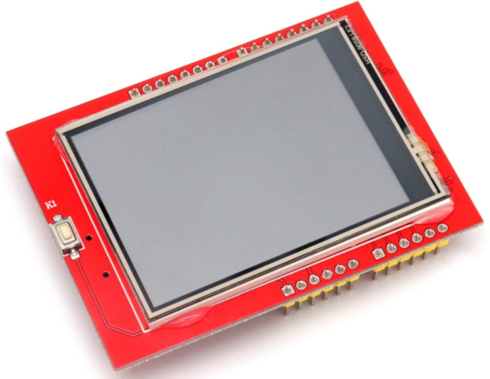
\includegraphics[scale=0.4]{figures/ili.png}
		\end{center}
		\caption{Lo schermo ILI9341.}
		\label{fig:ili9341}
	\end{subfigure}
\end{figure}

L'ultimo componente hardware necessario è la plancia di gioco: per questo
utilizziamo una board costruita appositamente per il form factor del GameBoy
originale con $12$ tasti. Ne abbiamo utilizzati solo $8$: frecce direzionali,
\texttt{A}, \texttt{B}, \texttt{SELECT} e \texttt{START}.

\begin{figure}[h]
	\begin{center}
		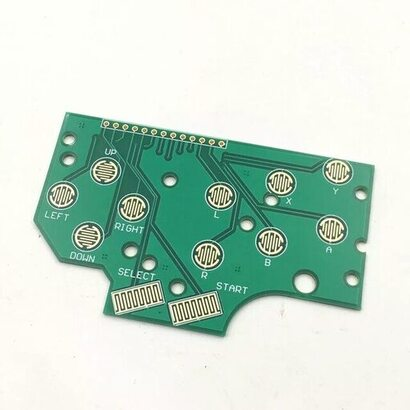
\includegraphics[scale=0.4]{figures/pcb.jpeg}
	\end{center}
	\caption{La PCB GB DMG.}
	\label{fig:pcb}
\end{figure}

\subsection{Materiali}

\begin{center}
	\begin{table}[h]
		\centering
		\begin{tabular}{|llll|l|}
			\hline
			\multicolumn{1}{|l|}{\textbf{Nome}}    & \multicolumn{1}{l|}{\textbf{Modello}}  & \multicolumn{1}{l|}{\textbf{Costo unitario}} & \textbf{Unità} & \textbf{Costo} \\ \hline
			\multicolumn{1}{|l|}{Guscio esterno}   & \multicolumn{1}{l|}{GB DMG-01 Shell}   & \multicolumn{1}{l|}{9.90}                    & 1              & 9.90           \\ \hline
			\multicolumn{1}{|l|}{Plancia di gioco} & \multicolumn{1}{l|}{GB DMG-01 PCB}     & \multicolumn{1}{l|}{1.18}                    & 1              & 1.18           \\ \hline
			\multicolumn{1}{|l|}{Bottoni}          & \multicolumn{1}{l|}{GB DMG-01 Buttons} & \multicolumn{1}{l|}{2.95}                    & 1              & 2.95           \\ \hline
			\multicolumn{1}{|l|}{Schermo}          & \multicolumn{1}{l|}{ILI9341 2.4"}      & \multicolumn{1}{l|}{6.44}                    & 2              & 12.88          \\ \hline
			\multicolumn{1}{|l|}{Microcontrollore} & \multicolumn{1}{l|}{STM32 F411CEU6}    & \multicolumn{1}{l|}{7.03}                    & 1              & 7.03           \\ \hline
			\multicolumn{1}{|l|}{Interruttore}     & \multicolumn{1}{l|}{SS12D00 4mm}       & \multicolumn{1}{l|}{0.30}                    & 1              & 0.30           \\ \hline
			\multicolumn{1}{|l|}{Millefori}        & \multicolumn{1}{l|}{50x70mm}           & \multicolumn{1}{l|}{3.50}                    & 1              & 3.50           \\ \hline
			\multicolumn{1}{|l|}{Cavi e stagno}    & \multicolumn{1}{l|}{-}                 & \multicolumn{1}{l|}{-}                       & 1              & 2.00           \\ \hline
			\multicolumn{4}{|r|}{\textbf{Totale}}  & 39.74€                                                                                                                  \\ \hline
		\end{tabular}
		\caption{
			Materiali utilizzati per la costruzione del progetto. I costi indicati
			provengono da negozi online come Amazon, eBay e Aliexpress
		}
	\end{table}
\end{center}

\subsection{Schema di collegamento}
Lo schema dei collegamenti è mostrato in \cref{fig:schema}.
\begin{figure}[h]
	\begin{center}
		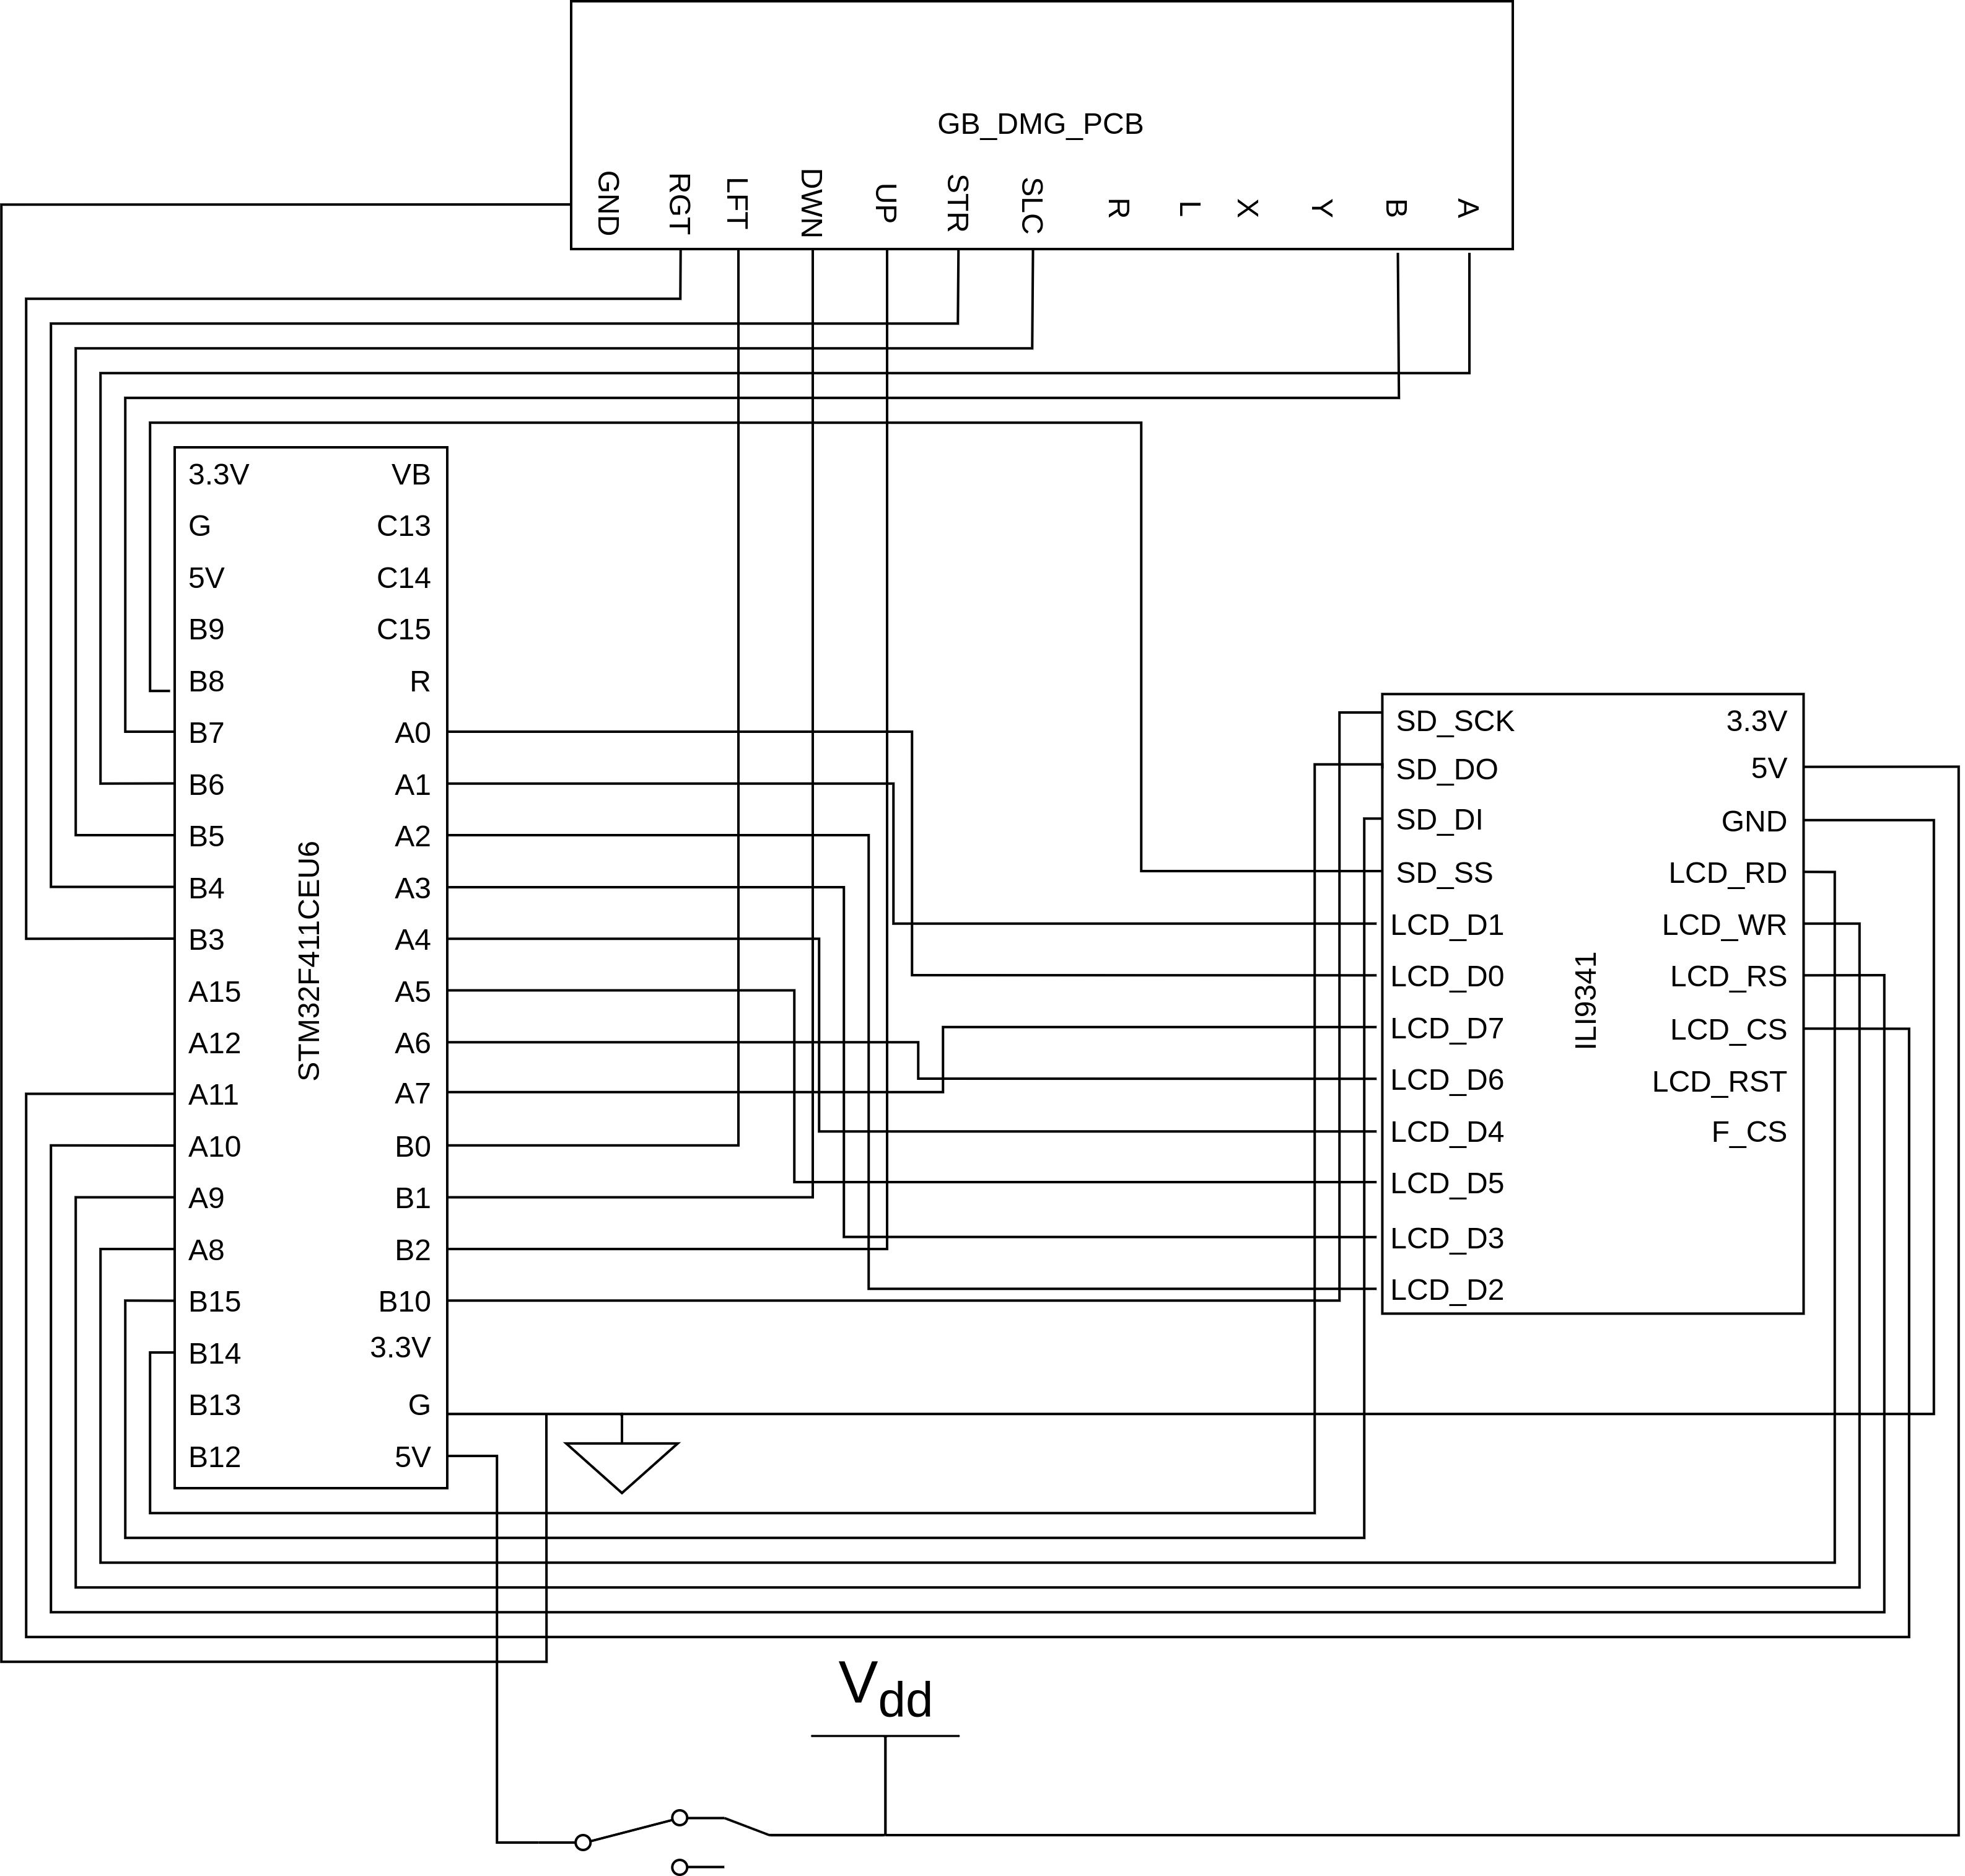
\includegraphics[scale=0.65]{figures/scheme.png}
		\caption{}
		\label{fig:schema}
	\end{center}
\end{figure}

\section{Software}
Il software necessario per il progetto si divide nei seguenti moduli: gestione
della scheda microSD, emulatore, interfaccia con lo schermo e una GUI per la
selezione dei giochi.

\subsection{Emulatore}
Il modo in cui il nostro progetto permette di eseguire videogiochi originali
del GameBoy è tramite l'emulazione. Un emulatore è un software che simula il
processore ed eventuali altre periferiche in modo di eseguire
programmi scritti per una certa architettura su un'altra architettura
potenzialmente diversa.
Scrivere un emulatore richiede uno studio attento dell'architettura che si
vuole emulatore ed è al di fuori dello scopo del corso, per questo motivo
abbiamo deciso di riutilizzare il codice di un emulatore già esistente ed
open source.

L'emulatore che abbiamo scelto è \texttt{peanutGB}, scritto in C e progettato
per essere facilmente portato su diverse piattaforme.
Questo emulatore è distribuito in un singolo file sorgente, non richiede
dipendenze e separa efficacemente il cuore dell'emulatore dalle interfacce di
input e output.
Per integrare questo emulatore nel nostro progetto è stato dunque necessario
implementare degli \textit{hooks} come per esempio \texttt{gb\_rom\_read},
\texttt{gb\_cart\_ram\_write} oppure \texttt{gb\_lcd\_draw\_line}.

Il porting di questo emulatore per il microcontrollore non ha richiesto
particolari modifiche. Nonostante questo, in generale, emulare una altra
architettura è una operazione piuttosto costosa dal punto di vista delle
performance, e il nostro caso non fa eccezione: allo scopo di misurare le
performance del nostro progetto, utilizziamo la misura di \textit{fotogrammi
per secondo} (FPS). 

Il GB originale aggiorna il proprio schermo circa 60 volte al secondo, dunque
idealmente per avere una emulazione a piena velocità il nostro microcontrollore
dovrebbe produrre $60$ FPS. Le performance variano in base alla complessità dei
giochi: la maggior parte dei giochi hanno un \textit{framerate} intorno a $55$
FPS, con qualche calo occasionale a $45$ FPS nei momenti più concitati.
Casi ``patologici'' sono alcuni dei giochi più complessi rilasciati verso il
fine vita della console hanno framerate più bassi, intorno a $35$ FPS; 
in generale, tuttavia, la gran parte dei giochi rimane comunque giocabile. 

Per non compromettere le performance ulteriormente, abbiamo deciso di rinunciare
all'audio: seppur il DMA ci avrebbe permesso di mandare l'audio ad uno speaker
senza intaccare troppo le performance, emulare il processore audio del GameBoy e
generare i samples da mandare via PWM sarebbe stato molto dispendioso.

\subsubsection{Colori}
Originariamente, il GB disegnava esclusivamente in \textit{grayscale}: ogni
oggetto (sfondo, dialoghi, sprites, transizioni...) è assegnato ad uno dei $4$
\textit{layer} che il GB offre, che viene ulteriormente diviso in $4$
\textit{variables}, come mostrato in \cref{table:gb_colors}.
Con il rilascio del \textit{Game Boy Color}, \textit{Nintendo} preparò una serie
di \textit{palette} di colori per permettere ai giochi rilasciati in bianco e nero
di diventare a colori. Queste palette sono semplicemente 4 colori in formato BGR565
per ognuno dei 4 layer supportati.

Abbiamo estratto alcune palette dei giochi più popolari ed implementato questo
meccanismo di conversione dei colori grayscale nel corrispondente colore della
palette del layer del momento.

\begin{table}[h]
	\begin{tabular}{|l|l|llll|}
		\hline
		\textbf{Layer} & \textbf{Descrizione di uso tipico}                    & \multicolumn{4}{l|}{\textbf{Variabili}}                                                          \\ \hline
		\textbf{BG0}   & Sfondo                                                & \multicolumn{1}{l|}{B1}                 & \multicolumn{1}{l|}{B2} & \multicolumn{1}{l|}{B3} & B4 \\ \hline
		\textbf{Win}   & Menu a finestra: stato, pausa, mappa, inventario, HUD & \multicolumn{1}{l|}{W1}                 & \multicolumn{1}{l|}{W2} & \multicolumn{1}{l|}{W3} & W4 \\ \hline
		\textbf{Obj0}  & Sprites principali                                    & \multicolumn{1}{l|}{–}                  & \multicolumn{1}{l|}{S2} & \multicolumn{1}{l|}{S3} & S4 \\ \hline
		\textbf{Obj1}  & Transizioni, sprites secondari                        & \multicolumn{1}{l|}{–}                  & \multicolumn{1}{l|}{P2} & \multicolumn{1}{l|}{P3} & P4 \\ \hline
	\end{tabular}
	\caption{Tabella dei colori per il GB (da
		\cite{GameBoyColors}).}
	\label{table:gb_colors}
\end{table}

\subsection{Scheda SD}
Fisicamente, la scheda microSD è inserita nello schermo ILI9341, che dispone di
un'apposita porta; per interfacciarci con essa, abbiamo deciso di formattare la
scheda con un filesystem FAT e utilizzare, come descritto in \cite{stm1721}, una
libreria per l'interazione con tali filesystem astratta dal livello di fisico di
I/O; abbiamo pertanto utilizzato un'ulteriore libreria per interfacciarci con
la scheda SD: questo meccanismo viene implementato utilizzando i pin esposti
dallo schermo e direttamente collegati alla microSD (\texttt{SD\_SCK},
\texttt{SD\_DO}, \texttt{SD\_DI}, \texttt{SD\_SS}) che permettono l'utilizzo
dell'interfaccia seriale della scheda.

\subsubsection{Caching dei settori}
Abbiamo osservato che durante l'esecuzione la lettura dei blocchi della SD
costituiva un collo di bottiglia per la performance, tanto da rendere
impossibile l'utilizzo della console. Sfortunatamente la grande maggioranza
dei giochi sono troppo grandi per essere caricati interamente in memoria RAM,
con alcuni giochi che addirittura arrivano a MB di dimensione.

Per mitigare questo problema abbiamo implementato un meccanismo di caching dei
dati letti dalla SD con una strategia ``Least Recently Used''.
Durante l'inizializzazione dell'emulatore viene creata in memoria una struct
\texttt{Cache} contenente una linked list in cui vengono salvati i contenuti
dei blocchi letti dalla della SD.
In questa struct vengono mantenuti anche i metadati necessari per
ritrovare il blocco utilizzato più recentemente e meno recentemente; questi dati
e la lista vengono aggiornati in base alle richieste, inserendo il blocco
richiesto più recentemente in cima alla lista e contestualmente rimuovere quello
richiesto meno recentemente.

Tramite misurazioni empiriche abbiamo ottenuto le performance migliori
utilizzando una dimensione dei blocchi di $512$ bytes, riservando $20$KB di
memoria RAM per la cache (dunque fino a $40$ blocchi caricati temporanemente).
Questo meccanismo di caching è un modulo fondamentale; senza di esso l'esecuzione
dei giochi diventa talmente lenta al punto da essere inaccettabile.

%\subsubsection{Scrittura dei salvataggi}
%Durante l'esecuzione dei giochi, gli utenti possono salvare i propri progressi
%in dei file appositi gestiti dall'emulatore. Invece di rallentare l'esecuzione ad
%ogni salvataggio,  abbiamo deciso di utilizzare una coda per scrivere i
%salvataggi in blocco. 

\subsection{Driver ILI9341}
Per interfacciarsi con lo schermo è stato necessario scrivere un driver
apposito: per questa componente in particolare abbiamo speso buona parte del
tempo necessario per il completamento del progetto. Lo schermo \texttt{ILI9341}
dispone per l'utilizzatore $5$ pin di controllo: \texttt{LCD\_RD},
\texttt{LCD\_WR}, \texttt{LCD\_RS}, \texttt{LCD\_CS}, ed \texttt{LCD\_RST}.
Questi pin vengono utilizzati per modificare lo stato della scheda, come
descritto nella documentazione ufficiale.
\begin{table}[h]
	\begin{verbatim}

  int ILI9341_Init(struct ILI9341_t *ili, struct ILI9341_Pin_t D7,
                 struct ILI9341_Pin_t D6, struct ILI9341_Pin_t D5,
                 struct ILI9341_Pin_t D4, struct ILI9341_Pin_t D3,
                 struct ILI9341_Pin_t D2, struct ILI9341_Pin_t D1,
                 struct ILI9341_Pin_t D0, struct ILI9341_Pin_t RST,
                 struct ILI9341_Pin_t CS, struct ILI9341_Pin_t RS,
                 struct ILI9341_Pin_t WR, struct ILI9341_Pin_t RD);

  [...]

  void ILI9341_DrawFramebufferScaled(struct ILI9341_t *ili, 
                 uint16_t framebuffer[]);
  \end{verbatim}
	\caption{}
	\label{table:driver_ili}
\end{table}
\subsubsection{Ad alto livello}
Nella \cref{table:driver_ili} mostriamo parte delle funzioni che, ad alto
livello, il driver implementa: ovviamente, \texttt{ILI9341\_Init} è utilizzata
per inizializzare l'unità; \texttt{ILI9341\_DrawFramebufferScaled}, anch'essa
abbastanza auto-esplicativa, è tra le funzioni del driver più utilizzate dal
codice utente per disegnare sullo schermo. Originariamente il GB mostrava uno
schermo $160\times144$: tra le migliorie che abbiamo implementate vi è anche lo
scaling dell'immagine dello schermo, che è aumentata a $320\times240$.

Esaminiamo ora l'implementazione di queste due funzioni; una struct mantiene lo
stato interno dei collegamenti tra microcontrollore e scheda, e tramite le
procedure offerte dal meccanismo GPIO di \texttt{HAL} possiamo impostare lo
stato dei pin dello schermo.

\subsubsection{Inizializzazione}
La funzione di inizializzazione è parametrizzata dagli identificatori dei pin
GPIO del microcontrollore che vengono collegati ai pin della scheda: una volta
inizializzata la struct che mantiene le corrispondenze di questi collegamenti,
si procede ad inizializzare i pin di controllo della scheda ( \texttt{LCD\_RD},
\texttt{LCD\_WR}, \texttt{LCD\_RS}, \texttt{LCD\_CS}, ed \texttt{LCD\_RST}) come
pin di output tramite le funzioni messe a disposizione da HAL. Diamo quindi uno
stato iniziale alla scheda prima di procedere alla sequenza di inizializzazione:
il pin \texttt{LCD\_CS} è impostato come \textit{attivo} (quindi \textit{low},
come da richieste della scheda). Questo significa che la scheda è pronta a
ricevere dei comandi inviati dal microcontrollore. Si imposta quindi come
disabilitato (ossia \textit{high}) il pin \texttt{LCD\_RST}: questo pin forza la
scheda ad eseguire il reset, pertanto durante tutta l'esecuzione (o finché non
si desidera resettare lo schermo) dovrà rimanere disabilitato.
Si impostano disablitati i pin \texttt{LCD\_WR} e \texttt{LCD\_RD}; infine si
imposta come attivo (quindi \textit{low}) il pin \texttt{LCD\_CD}, che sta a
significare che la scheda riceverà sui pin dati un comando.

L'effettiva sequenza di inizializzazione della scheda comporta l'attivazione del
pin \texttt{LCD\_RST} seguito da un delay  e la seguente disattivazione dello
stesso pin seguito da un ulteriore delay.

\subsubsection{Disegnare sullo schermo}
La funzione \texttt{ILI9341\_DrawFramebufferScaled} utilizza l'interfaccia della
scheda e il protocollo descritto nella documentazione per disegnare sullo
schermo. Nella nostra implementazione abbiamo scelto di utilizzare un framebuffer
globale sul quale emulatore e GUI disegnano.

\begin{figure}[h]
	\centering
	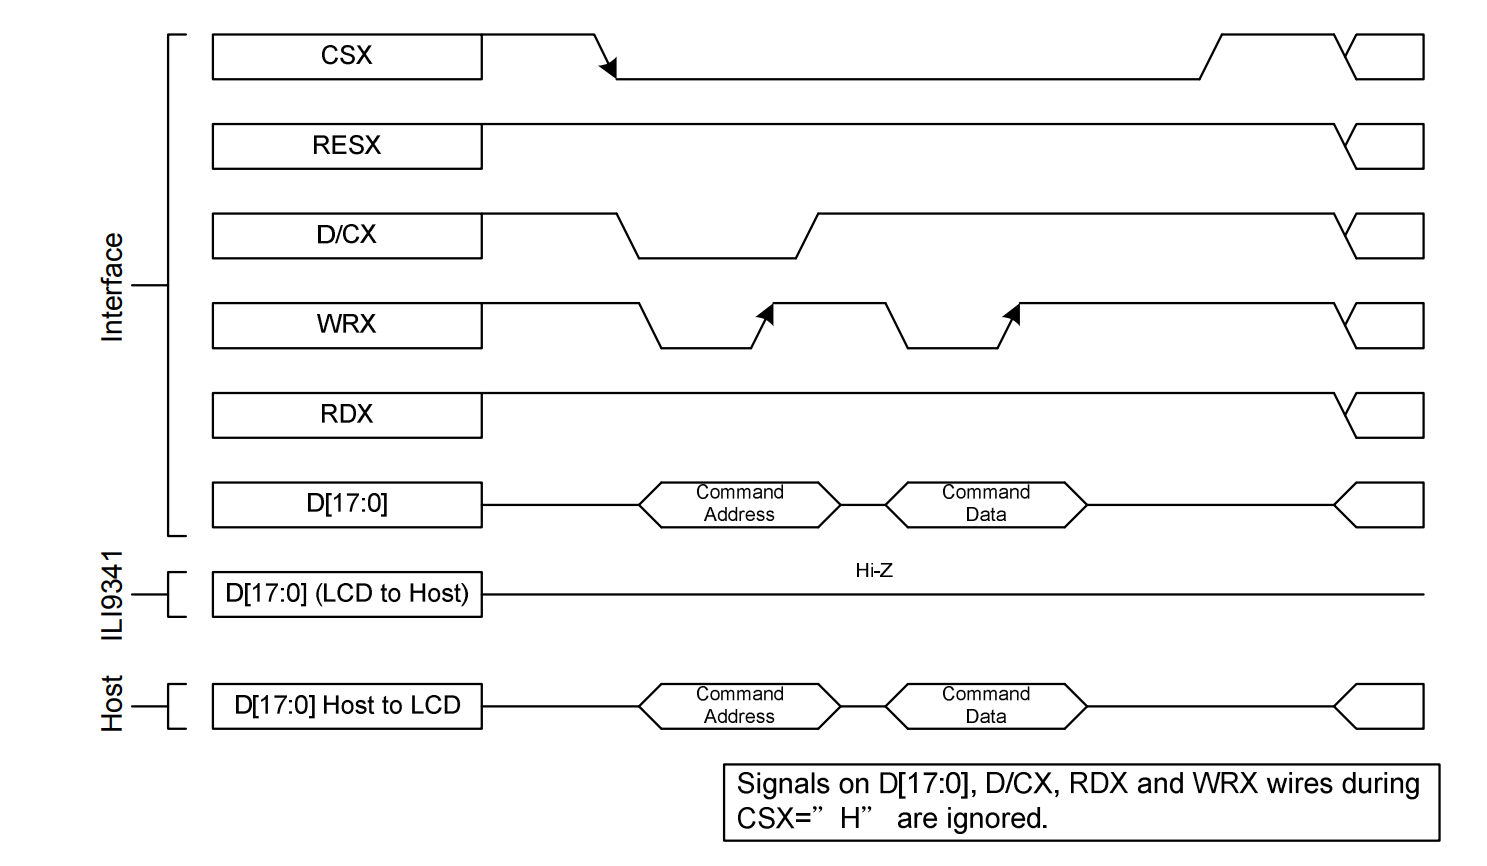
\includegraphics[scale=0.8]{figures/wr_cycle.png}
	\caption{}
	\label{fig:ili_wr_cycle}
\end{figure}

Per implementare il protocollo, la funzione imposta lo schermo per
la ricezione di comandi e invia inizialmente una \texttt{nop}, con lo scopo di
sincronizzare scheda e microcontrollore.

Il protocollo della scheda prevede che il client, per disegnare sullo schermo,
imposti inizialmente l'area sulla quale vuole disegnare.
L'utente dispone dei comandi \texttt{COLUMN\_ADDRESS\_SET} e
\texttt{PAGE\_ADDRESS\_SET}: il primo comando è utilizzato per specificare le
due colonne destra e sinistra che delimitano l'area in cui si vuole disegnare, e
simmetricamente fa il secondo comando; entrambi i comandi richiedono quattro
parametri da $8$bit che indicano i $2+2$ byte necessari per identificare righe e
colonne. Una volta specificata l'area, l'utente utilizzerà il comando
\texttt{MEMORY\_WRITE} per inviare alla scheda i dati che descrivono il disegno.
Ogni pixel dello schermo è descritto da due byte in formato BGR565 e verrà
inviato seguendo il \textit{write cycle} come descritto in
\cref{fig:ili_wr_cycle}.

Nell'implementazione abbiamo deciso di forzare l'utilizzo dei pin
\texttt{A0}-\texttt{A7} del microcontrollore per l'invio dei dati allo schermo
(ossia devono essere collegati ai pin \texttt{D0}-\texttt{D7} dello schermo): in
questo modo possiamo scrivere direttamente sul registro \texttt{GPIOA->ODR} il
byte da inviare. Possiamo dunque evitare l'utilizzo della HAL di ST e di
operazioni di \texttt{mask} e \texttt{shift}: questo ci permette di ottenere
prestazioni migliori evitando overhead non indifferenti.

\paragraph{Scaling}
L'algoritmo di scaling che abbiamo implementato cerca di scalare l'immagine
prodotta da GUI ed emulatore senza sacrificare le performance ed è pertanto
relativamente semplice: aggiungiamo un pixel ogni due, sia in verticale che in
orizzontale; il nuovo pixel avrà come colore la media dei colori dei due pixel
che lo hanno generato.

\subsection{GUI}
\begin{figure}[h]
	\begin{center}
		\begin{subfigure}[b]{0.4\textwidth}
			\begin{center}
				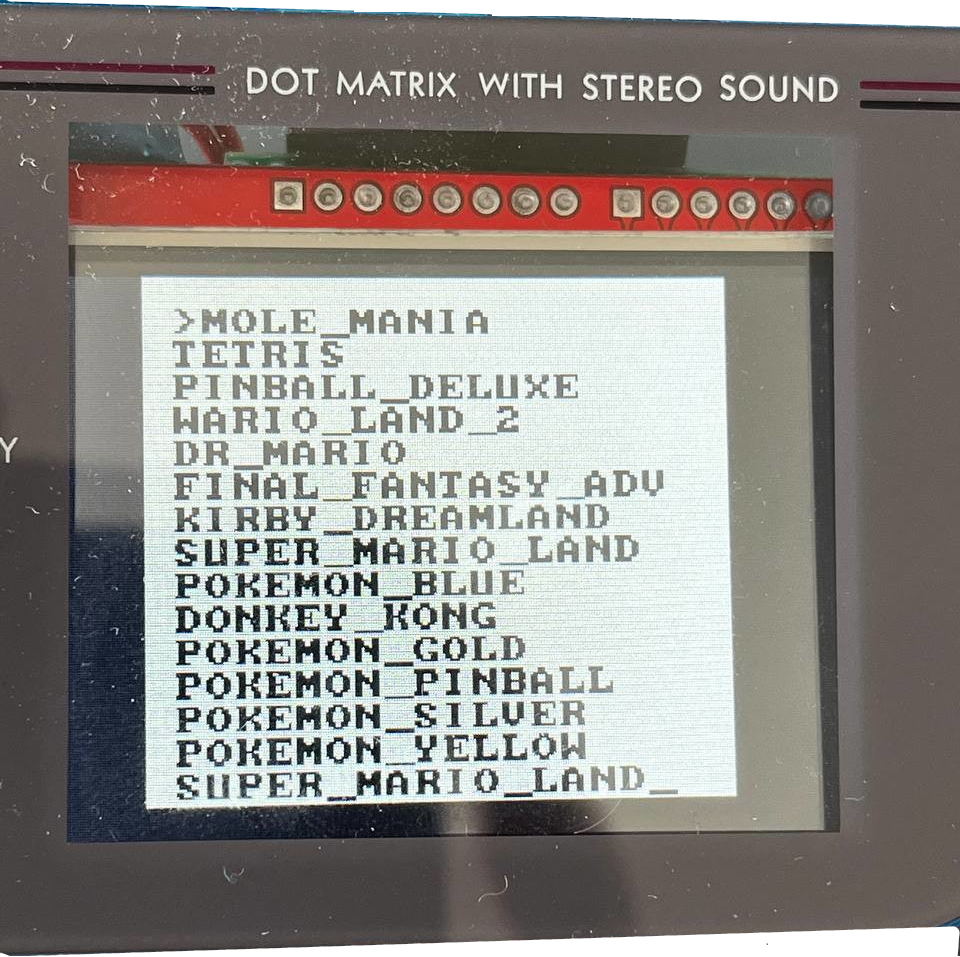
\includegraphics[scale=0.65]{figures/game_choice_gui.png}
			\end{center}
			\caption{}
			\label{fig:gui_choice}
		\end{subfigure}
		\hfill
		\begin{subfigure}[b]{0.4\textwidth}
			\begin{center}
				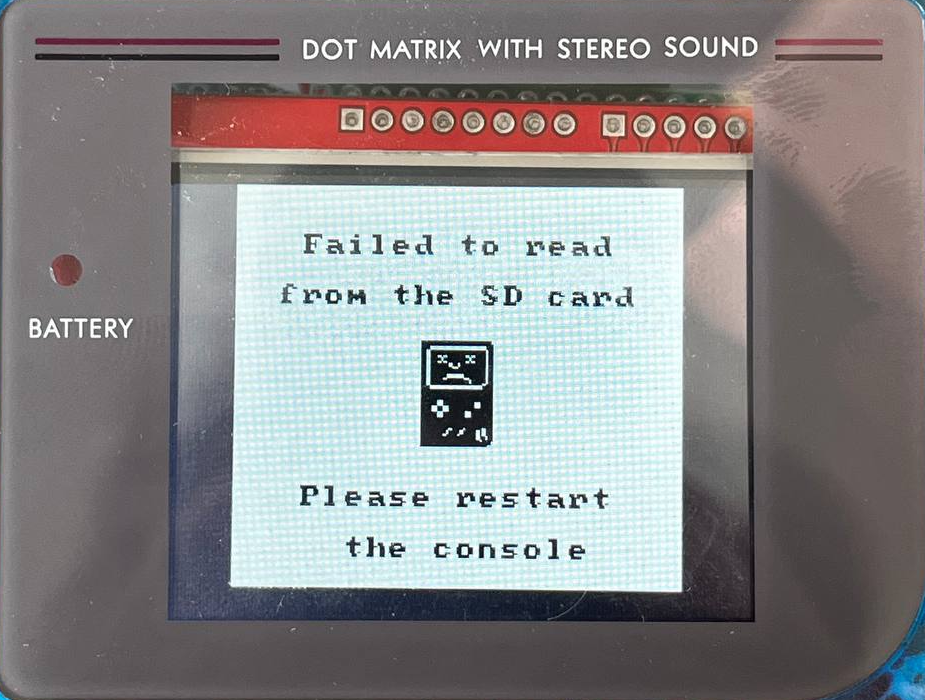
\includegraphics[scale=0.2]{figures/error_gui.png}
			\end{center}
			\caption{}
			\label{fig:gui_err}
		\end{subfigure}
	\end{center}
	\caption{}
\end{figure}
Abbiamo scritto una semplice GUI per permettere all'utente di scegliere i giochi
disponibili sulla scheda SD (\cref{fig:gui_choice}) o, in caso non vi siano
giochi disponibili sulla scheda SD (o non sia inserita) mostrare a schermo un
messaggio di errore (\cref{fig:gui_err}).
Benché siano disponibili diversi framework per sviluppare GUI su ambienti
embedded, abbiamo deciso di non utilizzarli implementando da zero il tutto, data
la relativa semplicità dell'interfaccia che abbiamo immaginato.

\subsubsection{Font PSF}
Questo componente software scrive direttamente i valori dei pixel nel
framebuffer globale. Per poter mostrare a video i nomi dei giochi disponibili è
necessario implementare la risoluzione di font sullo schermo: per fare questo
abbiamo utilizzato i font PSF che codificano ogni \textit{glifo} (ossia ogni
simbolo, ad esempio una lettera) come bitmap. Nel font che abbiamo scelto, i
simboli vengono codificati come $8$ righe di $8$ bit ciascuna: un bit $i = 0$
indica che per mostrare il glifo, il pixel corrispondente al bit $i$ deve avere
il colore di background dello schermo, mentre un bit $i = 1$ indica che il pixel
deve avere il colore di foreground. Assieme con queste bitmap, per implementare
la GUI sono bastate delle funzioni che svolgono dei  semplici calcoli sulle
dimensione del framebuffer (ossia calcolare i rettangoli in cui andare a
dipingere i glifi).
\begin{table}[h]
	\begin{verbatim}
// Character 48
Bitmap: -#####-- \
        ##---##- \
        ##--###- \
        ##-#-##- \
        ###--##- \
        ##---##- \
        -#####-- \
        --------
Unicode: [00000030];
	\end{verbatim}
	\caption{Il glifo ``0'' nel font PSF \texttt{koi8r} per l'alfabeto cirillico.}
\end{table}

\section{Assemblaggio}
Abbiamo speso una buona parte del tempo totale della realizzazione del progetto
a pianificare e tentare vari approcci per l'assemblaggio finale. Questa parte di
svolgimento, infatti, si è rivelata più ostica del previsto, poiché l'insieme
dei componenti e dei cavi non stava nel case del GB.

Essendo la PCB del gamepad un clone dell'originale del GameBoy, il case è
costruito per alloggiarla comodamente. Sfortunatamente non si può dire lo stesso
del nostro schermo e microcontrollore, essendo componenti completamente diversi
da quelli trovati nel GB originale, in cui l'intera circuiteria è posizionata
dietro lo schermo; in questo spazio il nostro display e microcontrollore
occupano l'intero spazio verticale, lasciando poco spazio per i cavi.

Il nostro primo tentativo di utilizzare dei semplici cavetti per i collegamenti
si è rivelato fallimentare: l'alto numero di collegamenti e il loro spessore
(anche dopo averli accorciati) rendevano difficilissimo chiudere il case.
Inoltre, anche dopo essere riusciti a chiudere il tutto, questi cavetti erano
proni a staccarsi dai pin durante la sessione di gioco.

La soluzione è stata quella di riprodurre i collegamenti su una millefori,
saldando dei cavetti piatti in stagno su di essa ed utilizzando dei pin header
femmina che fungono da alloggiamento per il microcontrollore.
Questa millefori, tagliata per essere delle stesse dimensioni dello schermo, è
stata progettata per essere saldata sui pin dello schermo, riducendo al minimo
lo spessore totale.

\begin{figure}[h]
	\begin{center}
		\begin{subfigure}[b]{0.4\textwidth}
			\begin{center}
				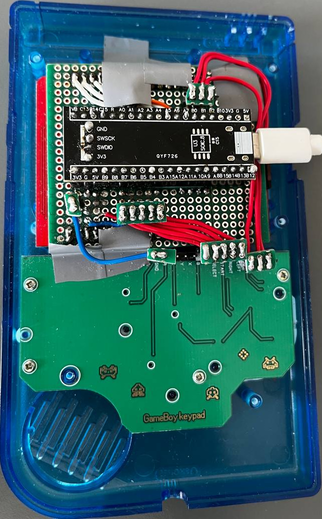
\includegraphics[scale=0.45]{figures/pcb_front.png}
			\end{center}
			\caption{}
			\label{fig:pcb_front}
		\end{subfigure}
		\hfill
		\begin{subfigure}[b]{0.4\textwidth}
			\begin{center}
				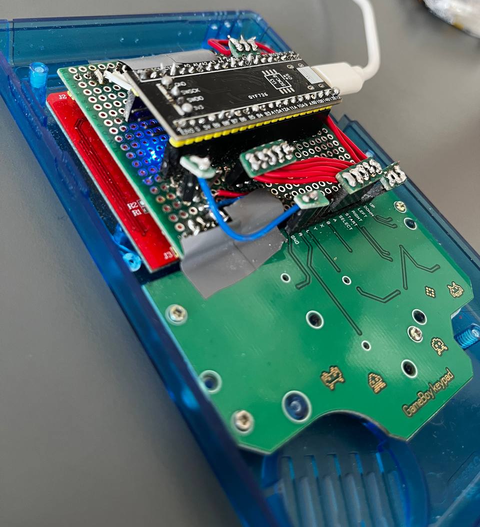
\includegraphics[scale=0.4]{figures/pcb_side.png}
			\end{center}
			\caption{}
			\label{fig:pcb_side}
		\end{subfigure}
	\end{center}
	\caption{}
\end{figure}


Questa millefori espone dei pin maschio per l'alimentazione (5V e GND)
e per i tasti (da PB0 a PB8), collegati direttamente ai pin del
microcontrollore.
Questi pin vengono collegati rispettivamente al cavi dell'alimentazione e
ai pin della PCB dei tasti.

In mezzo ai cavi che collegano batterie e microcontrollore troviamo un semplice
interruttore, che viene posizionato sulla parte superiore del GameBoy.
L'interruttore utilizzato è uno switch SPDT, dunque a singolo polo con doppia
mandata, ma noi utilizziamo solamente una delle due mandate. La scelta di
utilizzare uno switch a due mandate invece di uno con singola mandata è dovuto
al fatto che i primi sono molto più economici e reperibili dei secondi.
Lo switch ed i cavi a cui è collegato sono stato saldati su un piccolo pezzo
di millefori, tagliato per fare in modo che si incastri nelle incavature già
presenti nel case del GameBoy.


\subsection{Alimentazione e consumi}
La scheda che abbiamo scelto contiene al suo interno un regolatore di tensione
in input da $+3.52$V fino $+5.25$V: questo ci ha permesso di costruire un
sistema di alimentazione molto semplice, composto banalmente da 3 batteria AA
($1.5$V ciascuna) in serie per un totale di $+4.5$V in ingresso.

Abbiamo misurato che il nostro progetto consuma circa $116$mA. La conosole
originale, invece, ne consuma tra i $70$ e gli $80$. Assumendo che le batterie
in uso siano da $2500$mAh, utilizzando la formula 
$$
\text{tempo} = \frac{\text{capacità batteria}}{\text{consumo}} 
$$
otteniamo $2500/116 \approx 21$ ore come autonomia per il nostro progetto,
mentre per il GB è $2500/70 \approx 35$.

\section{Considerazioni finali}

Con rammarico ci tocca ammettere di aver sottostimato la potenza necessaria per
emulare questi videogichi, e di aver dovuto di conseguenza effettuare dei
compromessi significativi nella realizzazione finale; primo tra tutti l'assenza
del suono. Con il senno di poi sicuramente sceglieremmo una scheda più potente,
oppure opteremmo per emulare una console meno potente.

Nonostante questo, il fatto che molte persone a cui abbiamo fatto provare il
progetto riuscissero a perdersi in lunghe sessioni di gioco in \texttt{Tetris}
o \texttt{Super Mario Land} ci porta a dire di aver comunque raggiunto il
nostro obiettivo.


\addcontentsline{toc}{section}{References}
\nocite{*}
\printbibliography
\end{document}
